\chapter{Rijen}

We hebben tot nu toe variabelen gebruikt als string, als getal of als booleaanse waarden. Variabelen komen intern overeen met geheugenplaatsen in het geheugen van de computer.

Voorbeeld: var getal = 15; vanaf dit ogenblik zal overal waar we de naam getal gebruiken dit hetzelfde zijn als de numerieke waarde 15; tenzij we deze waarde ondertussen natuurlijk hebben gewijzigd. We kunnen de variabele getal namelijk gebruiken in instructies die de waarde van de variabele veranderen. Voorbeeld: de instructie getal = getal * 2;  zal ervoor zorgen dat de variabele getal nu de waarde 30 heeft.

Soms is het nodig om gegevens bij te houden in meer ingewikkelde gegevensstructuren. Een rij (\emph{Eng.: Array}) is hiervan een voorbeeld. Een array komt overeen met een vast aantal variabelen die allen van hetzelfde type zijn\footnote{Dit is niet iets wat door JavaScript afgedwongen wordt (in principe kunnen er in een array elementen staan van verschillende types), maar wij gaan enkel arrays gebruiken waarvan de elementen allemaal hetzelfde type hebben.}, dus alle elementen zijn getallen of alle elementen zijn booleaanse waarden of alle elementen zijn strings. Het aantal elementen van een array met naam rij wordt in JavaScript genoteerd door rij.length. Een array wordt in JavaScript gedeclareerd als volgt:

\examplecode{Rijen/creation.js}

met aantalElementen uiteraard >= 2 (dit is niet verplicht, maar een lijst met nul of \'e\'en elementen is zelden nuttig).

De array heeft in zijn geheel een naam (bijvoorbeeld naamRij) en we kunnen ook de individuele elementen benoemen, door de naam van de array gevolgd door `[' ,een index, en tenslotte een `]'. De elementen van een array met naam naamRij worden in JavaScript (en ook in Java, C++, \ldots) ge\"indexeerd vanaf 0..rij.length-1. Dus het $i^{de}$ element van een array met naam naamRij wordt genoteerd als naamRij[i].

Belangrijk is dat de elementen van een array niet alleen van dezelfde soort zijn, maar dat ze ook een zelfde betekenis hebben. Dus een array waarvan het eerste element de brilsterkte van de ene persoon bevat en het tweede element het IQ van een andere persoon bevat is niet toepasselijk.

Bijvoorbeeld: een student legt examen af van 10 verschillende vakken. Een examenresultaat wordt uitgedrukt door middel van een geheel getal groter of gelijk aan nul en kleiner of gelijk aan 20. De 10 examenresultaten van een student kunnen dan bijgehouden worden in een array met naam examenResultaten van 10 getallen:

\examplecode{Rijen/example.js}

examenResultaten[5] zal dan het examenresultaat bevatten van het zesde vak dat de student heeft afgelegd; examenResultaten.length zal gelijk zijn aan 10.

Je kan de elementen van een array ook opsommen op het ogenblik van declaratie als volgt (er zijn twee alternatieve notaties die hetzelfde effect hebben):

\examplecode{Rijen/literal.js}

Voorbeeld:

\examplecode{Rijen/literalexample.js}

Code om een array te manipuleren zal dikwijls gebruik maken van for-lussen omdat de besturingsvariabele hier de rol kan spelen van index. Bijvoorbeeld: in volgend stukje code wordt het aantal buizen van een student berekend:

\examplecode{Rijen/buizen.js}

Uit voorgaande blijkt dat arrays kunnen meegegeven worden als parameter. Arrays kunnen ook teruggegeven worden als teruggeefwaarde in een functie. Voorbeeld:

\examplecode{Rijen/draaiom.js}

Bekijk volgend stukje code:

\examplecode{Rijen/keerom.js}

Wanneer je nu de array aRij element per element uitschrijft zal je merken dat de elementen van aRij omgekeerd zijn dus [5,4,3,2,1]. Dit komt omdat wanneer je een array als parameter doorgeeft eigenlijk het adres van het eerste element wordt gekopieerd in de parameter; de adressen van de volgende elementen worden dan berekend op basis van dit eerste adres omdat de geheugenplaatsen van de verschillende elementen fysisch mekaar opvolgen. Dit betekent concreet in ons voorbeeld dat rij[i] en arij[i] eigenlijk namen zijn van dezelfde variabelen. Dus wanneer je iets wijzigt aan rij[i] binnen het instructiegedeelte van de functie zal er dan ook een analoge wijziging gebeuren aan aRij[i]!

\section{Werken met arrays in JavaScript}

Arrays zijn heel belangrijk in JavaScript, en daarom zijn er een aantal JavaScript-methodes die speciaal gebruikt kunnen worden om het werken met arrays te vereenvoudigen. We bespreken hier kort de meest interessante methodes. Voor een uitgebreide lijst, zie \url{http://www.w3schools.com/jsref/jsref_obj_array.asp}

\subsection{Push en pop}

Pop verwijdert het laatste element van de array, en geeft het verwijderde element als teruggeefwaarde. Push voegt een element op het einde van een array toe.

\examplecode{Rijen/pushpop.js}


\subsection{Shift en unshift}

Shift verwijdert het eerste element van de array, en geeft het verwijderde element als teruggeefwaarde. Unshift voegt een element aan het begin van een array toe.

\examplecode{Rijen/shiftunshift.js}


\subsection{Slice}

Slice gaat een aantal elementen selecteren uit een array. De methode verwacht twee parameters: de index van het element waar de selectie begint, en de index van het element waar de selectie eindigt (exclusief dit laatste element!).

\examplecode{Rijen/slice.js}


\subsection{Splice}

Splice kan een aantal elementen in het midden van de rij toevoegen of verwijderen. Splice heeft 2 verplichte parameters en dan onbeperkt aantal optionele parameters. De eerste parameter geeft aan waar in de rij je elementen wilt toevoegen of verwijderen. De tweede parameter geeft aan hoeveel elementen je wilt verwijderen (0 voor toevoegen). Vanaf de derde parameter geef je aan welke de extra toe te voegen elementen zijn.

\examplecode{Rijen/splice.js}l

\subsection{Concat}

Concat gaat twee of meerdere arrays samenvoegen tot \'e\'en array. De methode verwacht als parameters \'e\'en of meerdere arrays en geeft als teruggeefwaarde het samengevoegde resultaat.

\examplecode{Rijen/concat.js}


\section{Zoekalgortimes}

Stel dat je wenst een functie te schrijven om te zoeken of een bepaalde waarde voorkomt  in een rij. Dit kan je op een aantal verschillende manieren doen, afhankelijk van of de rij gesorteerd is of niet.

\subsection{Lineair zoeken in een niet-gesorteerde rij}

Je vergelijkt het te zoeken element met alle elementen van de rij beginnend vanaf de eerste tot de laatste of tot je het gevonden hebt.

\examplecode{Rijen/zoeklin.js}

Zoektijd: N (met N het aantal elementen van de rij)

\subsection{Lineair zoeken in een gesorteerde rij}

Wanneer de rij gesorteerd is (van klein naar groot, of alfabetisch in het geval van een rij van Strings) dan hoef je wanneer de waarde niet voorkomt niet tot het laatste element van de rij te zoeken, maar kan je als je een element tegenkomt dat strikt groter is dan de te zoeken waarde al stoppen met zoeken.

\examplecode{Rijen/zoeklinsort.js}

Gemiddelde zoektijd: N/2 (met N aantal elementen van de rij)

\subsection{Binair zoeken in een gesorteerde rij}

Het binair zoekalgoritme werkt enkel bij een gesorteerde rij en werkt als volgt:

\begin{itemize}
\item[a] Je vergelijkt de te zoeken waarde met het middelste element
\item[b] Indien het gelijk is dan heb je het gevonden
\item[c] Indien het kleiner is dan beperk je je zoekinterval tot de eerste helft van de rij en ga je terug naar a
\item[d] Indien het groter is dan beperk je je zoekinterval tot de tweede helft van de rij en ga je terug naar a
\end{itemize}

Bij elke stap zal je zoekinterval halveren en de gemiddelde zoektijd is dan ook $log_{2}N$

\examplecode{Rijen/binzoek.js}

\section{Meerdimensionale Rijen}

Zoals in het begin van dit hoofdstuk opgemerkt werd, kunnen de elementen van een array eender welk type van variabele bevatten. Naast de booleaanse waardes (true en false), getallen en tekst, kan je dus ook een array in een array steken.

Stel dat we bijvoorbeeld de volgende code uitvoeren:

\examplecode{Rijen/multi.js}

De eerste twee lijnen maken elk een \'e\'en-dimensionale rij (zoals we tot nu toe altijd gebruikt hebben). De derde lijn maakt een nieuwe rij aan met de eerste twee rijen als elementen in de rij. In het geheugen ziet de rij er dus uit als in Figuur~\ref{fig:rij2dim}.

\begin{figure}
\centering
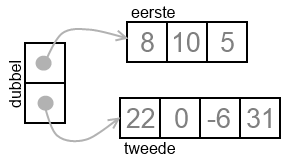
\includegraphics[scale=0.8]{Rijen/rij2dim.png}
\caption{Een tweedimensionale rij}\label{fig:rij2dim}
\end{figure}

Het eerste element van dubbel - element 0 - wijst naar rij eerste, terwijl het tweede element naar de rij tweede wijst. We kunnen nu elementen aanspreken als volgt:

\examplecode{Rijen/multi2.js}

De variabele getal zal nu als inhoud de waarde -6 krijgen, of de waarde die op de derde plaats (index 2 dus) opgeslagen zit van de tweede array (die met index 1) in dubbel. We kunnen de inhoud van de eerste array in dubbel als volgt aanpassen:

\examplecode{Rijen/multi3.js}

Bovenstaande code kwadrateert de waarde van i, en steekt dit resultaat dan in de eerste array van dubbel. Merk ook op dat we de lengte van de eerste array kunnen opvragen met de code dubbel[0].length. De waarde dubbel[0] is natuurlijk zelf een array, dus alle methodes die gedefinieerd zijn op rijen kunnen ook hier gebruikt worden.

We kunnen dezelfde originele tweedimensionale array ook krijgen op \'e\'en van de volgende alternatieve manieren:

\examplecode{Rijen/multilit.js}

Een tweedimensionale lijst kan gebruikt worden bij het oplossen van heel wat problemen. Stel bijvoorbeeld dat je een jaarlijkse kwisavond organiseert waar jij de software schrijft om het spel te beheren. Er zijn 10 ploegen zijn ingeschreven waar je de namen van bijhoudt in een \'e\'endimensionale rij:

\examplecode{Rijen/ploegen.js}

Er zijn 10 rondes; elke ploeg neemt deel aan elke ronde en behaalt hier een score >= 0 en <= 50. Dit resulteert in 100 getallen die we kunnen organiseren in 10 keer 10 getallen: dus voor elke ploeg 10 getallen met de score behaald op elke ronde.

Dit is een tweedimensionale rij van getallen. Het wordt ook wel een homogene tweedimensionale rij genoemd omdat alle elementen van hetzelfde type zijn en een zelfde betekenis hebben namelijk de score behaald door een bepaalde ploeg tijdens een bepaalde ronde.

\examplecode{Rijen/scores.js}

Dus scores is een rij bestaande uit 10 elementen en elk element is opnieuw een rij bestaande uit 10 getallen. scores[5][6] bevat dan het resultaat behaald door de zesde ploeg tijdens de zevende ronde.

Een rij van rijen noemen we een tweedimensionale rij. In het algemene geval kunnen we N-dimensionale rijen maken met N eender welk positief natuurlijk getal. Zo is een driedimensionale array bijvoorbeeld een rij van rijen die rijen bevatten. Stel dat we een filmpje in een array willen opslaan. Elk beeld van het filmpje is een tweedimensionale rij van pixels, en de lijst van beelden is dan een driedimensionale array. Figuur~\ref{fig:rij3dim} toont een voorbeeld waarbij de waarde beelden[0][x][y] de pixel teruggeeft op locatie (x, y) van het eerste beeld. In de praktijk gaan we vooral rijen gebruiken van \'e\'en of twee dimensies.

\begin{figure}
\centering
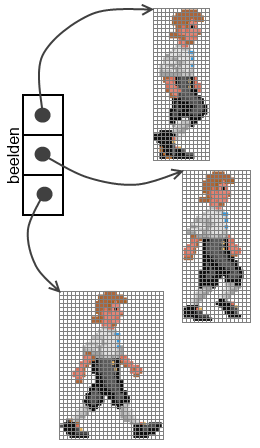
\includegraphics[scale=0.8]{Rijen/rij3dim.png}
\caption{Een driedimensionale rij}\label{fig:rij3dim}
\end{figure}


%%% Local Variables: 
%%% mode: latex
%%% TeX-master: "../main"
%%% End: 
